\chapter {Marco teórico}
\section {Sistemas de recomendación}
  Un sistema de recomendación proporciona a los usuarios una conjunto de sugerencias personalizadas las cuales podemos catalogarlas como recomendaciones, dichas recomendaciones son sobre un determinado tipo de los cuales son llamados artículos. Los sistemas de recomendación estudian las características de cada usuario y mediante un procesamiento de los datos, encuentra un subconjunto de artículos que pueden resultar de interés para el usuario. Clasificación Los sistemas de recomendación (SR) se clasifican en 3 tipos: SR con Filtrado basado en Contenido: Las recomendaciones están basadas en el conocimiento que se tiene sobre los artículos que el usuario a proporcionado, pueden ser de forma implícita o explícita, y se le recomendarán artículos similares que le puedan gustar o interesar. SR basado en Filtrado Colaborativo: El filtrado colaborativo consiste en ver que usuarios son similares al usuario activo (o usuario al que hay que realizarle las recomendaciones) y después recomendar aquellos artículos que no han sido votados por el usuario activo y que han resultado bien valorados por los usuarios similares. SR con métodos de Filtrado Híbrido: Mezclan alguno de los dos filtrados mencionados anteriormente para realizar recomendaciones e incluso lo combinan con alguna otra técnica de inteligencia artificial como pueda ser la lógica borrosa o la computación evolutiva. \cite{10}

\section{API}
  Interfaz de programación de aplicaciones, abreviada como API (Aplication Programming Iterface, del ingles). El cual es un conjunto de especificaciones, subrutinas, funciones y procedimientos que las aplicaciones deben seguir para establecer una comunicación con otro software como una capa de abstracción por medio de ciertas llamadas a bibliotecas el cual sirven como interfaz entre diversos programas el cual consiste en proporcionar un conjunto de funciones de uso general, dicha interfaz le facilitara al usuario la interacción con el software. El uso de la API se da por lo regular cuando se quiere estandarizar una plataforma, además se pueden estipular unas APIs comunes a los que se deben acoplarse todos los desarrolladores de aplicaciones. 

  \subsection{API select}
    Las API select son aquelllas las cuales regresan un registro para una entidad, no actualice la base de datos. Como ya se menciono las API select sólo nos devuelven un solo registro, ademas necesita que se le pasen atributos de clave exclusivos en formato XML como entrada. Si un atributo de clave exclusivo no pasa en el XML de entrada, la API utiliza blancos para estos atributos en los criterios para seleccionar el registro. Puede haber más de una combinación de claves exclusivas y en dicha combinación, debe pasar una de las múltiples combinaciones. 

  \subsection{API List}
    Normalmente con el prefijo \"get\", las API list devuelven una lista de los registros para una entidad que coinciden con los criterios especificados en el XML de entrada, por mencionar un ejemplo, la API getOrderList() es aquella que nos devolverá una lista de órdenes. Si algún elemento en el XML de entrada contiene un valor en blanco, este elemtno será parsado en alto.Cabe mencionar y debemos mencionar que las API list no actualizan la base de datos. También podemos obtener los datos paginados de una API list, esto será llamando a la API getPage y pasando la API list como entrada a la API getPage. API update Las API update son aquellas que insertan nuevos registros en la base de datos. Ademas de que modifican o suprimen registros existentes en dicha base de datos. Las API update que modifican o eliminan los registros ya existentes son aquellas que utilizan la misma lógica que las API select para identificar qué registros son los que ha qye modificar . Si dicho registro no es encontrado, las API update generan una excepción. API REST Primeramente vamos a describir que es REST, REST significa REpresentational State Transfer, el cuál es un tipo de arquitectura para el desarrollo web el cual se apoya totalmente en el estándar HTTP. REST nos permitirá crear servicios y/o aplicaciones que se pueden implementadas por cualquier dispositivo o cliente, la única condición es que entienda el HTTP. Una REST API es una API, o librería de funciones, por la cual se accede por el protocolo HTTP. Mediante esta API se accede a través de direcciones web o URLs por la cual se enviaran los datos de nuestra consulta. Como respuesta a la consulta sobre el REST API se obtienen datos en distintos formatos, como pueden ser texto plano, XML, JSON, por mencionar algunos. 

\section{Bases datos orientadas a grafos}
 Hasta 1999 los motores de búsqueda evaluaban cada página web como una entidad autónoma, ordenándolas en base al contenido, sin prestar atención al resto de páginas. Pero en 1999 Google adoptó PageRank, creado por Larry Page, y que constituye un conjunto de algoritmos que evalúan las páginas webs en relación con otras páginas. \cite{12}

\subparagraph{Características}
No hay índices clásicos en las bases de datos basadas en grafos. Por el contrario, cada objeto almacenado es representado por nodos (entidades) y aristas (relaciones). Un nodo es un registro único que tiene al menos una propiedad. Las aristas definen las relaciones entre los nodos y los nodos y sus relaciones tienen a su vez predefinidas conjuntamente propiedades. Los nodos pueden tener múltiples aristas que definen los diferentes tipos de relaciones que tienen con otros nodos.

Las consultas en las bases de datos orientadas a grafos están diseñadas para empezar en un nodo específico y explorar sus relaciones con otros nodos. Un ejemplo podría ser “Qué libros están leyendo mis amigos que yo aún no haya leído”. Es por eso que este tipo de bases de datos están frecuentemente asociadas con motores de recomendación que se usan con frecuencia en aplicaciones sociales y de comercio electrónico.

A medida que las búsquedas se van haciendo más complejas, el tiempo de procesamiento va aumentando. Es por eso que las bases de datos basadas en grafos aprenden e indexan las relaciones más comunes con el objetivo de acelerar el tiempo de búsqueda. \cite{13}
\subsection{Ventajas\cite{14}}
\begin{itemize}
  \item Rapidez para conectar datos. En las bases de datos relacionales, el frecuente uso de joins hace que las búsquedas sean lentas.
  \item Sencillez de las consultas.
  \item Rapidez en el manejo de consultas complejas que implican múltiples niveles de datos relacionados.
\end{itemize}
\subsection{Desventajas \cite{15}}
\begin{itemize}
  \item La búsqueda de nodos en diferentes máquinas puede ralentizar el proceso drásticamente.
  \item Requiere un cambio conceptual para los desarrolladores, por lo que implica una curva de aprendizaje.
\end{itemize}

\section{Neo4J}
Neo4j es una base de datos open-source orientada a grafos, esta escrita en java 1.2 y pertenece a este tipo de base de datos NoSQL.Los desarrolladores describen a Neo4j como un motor de persistencia embebido, basado en disco, completamente transactional Java que almacena datos estructurados en grafos más que en tablas. La versión 1.0 de Neo4j fue lanzada en febrero de 2010. La base de datos está licenciada en un modelo dual, tanto bajo Affero General Public License (AGPL) v3 como bajo licencia comercial.
Las bases de datos NOSQL son un conjunto de bases de datos que no se ajustan al modelo de bases de datos relacionales y sus características, estas no tienen esquemas  , no usan SQL ni permiten joins, no garantizan la propiedad ACID,  escalan horizontalmente, hacen uso amplio de la memoria principal del computador, resuelven el problema de los altos volúmenes de información y la inmensa cantidad de consultas y transacciones diarias, en resumen no son relacionales. \cite{16}
\subsection{Hay varios tipos de base de datos NOSQL: \cite{17}}
\begin{itemize}
	\item Orientada a columnas
	\item Clave-Valor
	\item Big Table
	\item Orientada a documentos
	\item Orientada a grafos
\end{itemize}
\subsection{Cómo Funciona Neo4j}
Neo4j usa grafos para representar datos y las relaciones entre ellos. Un grafo se define como cualquier representación gráfica formada por vértices (se ilustran mediante círculos) y aristas (se muestran mediante líneas de intersección). Dentro de estas representaciones gráficas, tenemos varios tipos de grafos:\cite{18}
\subsubsection{ Grafos no dirigidos:}
	 los nodos y las relaciones son intercambiables, su relación se puede interpretar en cualquier sentido. 	Las relaciones de amistad en la red social Facebook, por ejemplo, son de este tipo. 
\subsubsection{ Grafos dirigidos:}
	 los nodos y la relaciones no son bidireccionales por defecto. Las relaciones en Twitter son de este      	tipo. Un usuario puede seguir a determinados perfiles en esta red social sin que ellos le sigan a él.

\subsubsection{Grafos con peso:}
	en este tipo de gráficas las relaciones entre nodos tienen algún tipo de valoración numérica. Eso permite luego hacer operaciones.
\subsubsection{Grafos con etiquetas:}
	estos grafos llevan incorporadas etiquetas que pueden definir los distintos vértices y también las relaciones entre ellos. En Facebook podríamos tener nodos definidos por términos como ‘amigo’ o ‘compañero de trabajo’ y la relaciones como ‘amigo de’ o ‘socio de’.
\subsubsection{Grafos de propiedad}
	es un grafo con peso, con etiquetas y donde podemos asignar propiedades tanto a nodos como relaciones (por ejemplo, cuestiones como nombre, edad, país de residencia, nacimiento). Es el más complejo.
	Neo4j utiliza grafos de propiedad para extraer valor añadido de los datos de cualquier empresa con gran rendimiento y de una forma ágil, flexible y escalable.
\newpage
\subsubsection{Características de Neo4j\cite{19}}
Neo4j tiene las siguientes carácteristicas:
\begin{itemize}
	\item No hay esquema
	\item Transacciones ACID
	\item Puede contener billiones de nodos y relaciones
	\item Rápido recorriendo relaciones, este tipo de queries se conoce como transversals
	\item Lenguaje de query propio, Cypher
	\item Alta disponibilidad, instalación en diferentes maquinas con balanceador de carga
	\item Multilenguaje, proporciona una Api Rest pudiendo utilizarse desde cualquier lenguaje. Lenguaje drivers 			disponibles
\end{itemize}

\subsubsection{Procesamiento en grafo de forma nativa (Native Graph processing)}
    Tiene index-free adjancency, cada nodo tiene una referencia directa a su nodo adyacente, esto provoca    que el tiempo de una query no depende del tamaño total de la base de datos sino al área de búsqueda del grafo.\cite{20}
\subsubsection{Almacenamiento en grafo de forma nativa (Native Graph Storage)}
 	Hay ficheros para nodos, relaciones y propiedades. Al estar las propiedades de cada nodo y relación almacenado en un fichero diferente, el almacenamiento de nodos y relaciones se preocupa sólo de la estructura del grafo. Los tamaños son fijos y se puede obtener rápidamente en memoria nodos en base a su id, porque se sabe exactamente en que posición se encuentra este.\cite{21}
\newpage
 \subsection{Rendimiento}
	 Las bases de datos orientadas a grafos como Neo4j tienen mejor rendimiento que las relacionales (SQL) y las no relacionales (NoSQL). La clave es que, aunque las consultas de datos aumenten exponencialmente, el rendimiento de Neo4j no desciende, frente a lo que sí sucede con las BD relacionales como MySQL.
 	 Las BDOG responden a las consultas actualizando el nodo y la relaciones de esa búsqueda y no todo el grafo completo. Eso optimiza mucho el proceso.\cite{22}
\subsection{ Agilidad:}
	 Neo4J tiene muchas ventajas, pero una es su agilidad en la gestión de datos. Si nosotros quisiéramos llevar al límite sus capacidades, tendríamos que superar un volumen total de 34.000 millones de nodos (datos), 34.000 millones de relaciones entre esos datos, 68.000 millones de propiedades y 32.000 tipos de relaciones. \cite{23}
\subsection{Flexibilidad y escalabilidad:}
 	 Cuando los desarrolladores de una empresa trabajan con grandes datos, buscan flexibilidad y escalabilidad. Las bases de datos orientadas a grafos aportan mucho en este sentido porque cuando aumentan las necesidades, las posibilidades de añadir más nodos y relaciones a un grafo ya existente son enormes.\cite{24}
\subsection{Casos de uso de Neo4j}
\subsubsection{Recomendaciones en tiempo real y redes sociales:}
	Neo4j permite conectar de forma eficaz a las personas con nuestros productos y servicios, en función de la información personal, sus perfiles en redes sociales y su actividad online reciente. En este sentido, las bases de datos orientadas a grafos son interesantes porque son capaces de conectar personas e intereses.
	Con esa información, una empresa puede ajustar sus productos y servicios a su público objetivo y personalizar las recomendación en función de los perfiles. Eso es lo que permite que se aumente la precisión comercial y el compromiso del cliente.\cite{25}
\newpage
\section{Algoritmos de recomendación}
\subsection{k-Vecinos más cercanos (k-Nearest Neighbors)}
	El método k-nn (K nearest neighbors Fix y Hodges, 1951) es un método de clasificación supervisada. es un método de clasificación no paramétrico, que estima el valor de la función de densidad de probabilidad o directamente la probabilidad a posteriori de que un elemento x pertenezca a la clase Cj a partir de la información proporcionada por el conjunto de prototipos. En el proceso de aprendizaje no se hace ninguna suposición acerca de la distribución de las variables predictoras.\\ 
	\\
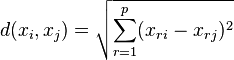
\includegraphics[width=0.3\textwidth, height=15mm]{images/formula}
\subsection{Slope One}
	El filtrado colaborativo es una técnica usada por los Sistemas de Recomendación para combinar las opiniones y pruebas de diferentes usuarios con el fin de obtener recomendaciones personalizadas. Hay al menos dos clases de filtrados colaborativos: las técnicas basadas en usuarios son derivadas de la medición de similitudes entre usuarios, mientras que las técnicas basadas en artículos comparan las valoraciones dadas por distintos usuarios. Slope One es una familia de algoritmos usados para el Filtrado Colaborativo introducida en Slope One Predictors for Online Rating-Based Collaborative Filtering por Daniel Lemire y Anna Maclachlan. Posiblemente, esta es la forma más simple de filtrado colaborativo basado en artículos. Su simplicidad la hace especialmente sencilla de implementar eficientemente mientras que su exactitud está a la par de algoritmos más complejos y costosos.
\subsection{Basado en Contenido}

Los sistemas de recomendación basados en contenido, emplean técnicas de recuperación de información. Por ejemplo, un documento de texto es recomendado basado en una comparación ente su contenido y el del perfil del usuario. Típicamente, el perfil muestra una lista de palabras clave y sus pesos correspondientes. Dicho perfil puede ser definido explícitamente, el usuario contesta cuestionarios, o de forma semiautomática en base a diversas heurísticas [Lieberman et al. 1997]. Para identificar el tema del documento se hace un análisis de frecuencia para extraer las palabras clave. Si a un usuario le gusta un documento, los pesos de las palabras extraídas se añaden a los pesos de las palabras correspondientes en el perfil del usuario. Este proceso es conocido como retroalimentación de relevancia [Balavanovic y Shoham 1997].

Este método de recomendación presenta algunos problemas como la sobre-especialización; el sistema sólo muestra al usuario elementos similares a los que ya ha visto anteriormente. Algunas veces este problema es resuelto agregando a la búsqueda aleatoreridad (por ejemplo mediante algoritmos genéticos). Otro problema se presenta al encontrar información multimedios, (con frecuencia presente en páginas de Web) puesto que cuando las recomendaciones son hechas sobre documentos de texto, está información es ignorada.
\newpage
\subsection{Filtrado colaborativo}
Estos sistemas de recomendación presentan elementos que le han gustado a otros usuarios con gustos similares, con este propósito, calculan la similitud entre usuarios. En estos sistemas el usuario debe realizar una evaluación previa sobre algunos elementos. De esta forma se va formando el perfil del usuario.Para cada usuario se crea un conjunto de "vecinos cercanos", usuarios cuyas evaluaciones anteriores tienen grandes semejanzas a las del usuario en cuestión. Los resultados para los elementos no calificados se predicen en base a la combinación de puntos (scores) conocidos de los vecinos cercanos.


En el filtrado colaborativo, el sistema no analiza los elementos evaluados, sino que las recomendaciones se basan solamente en la similitud entre usuarios. Esto trae consigo algunos problemas, como se comenta a continuación. Cuando un usuario llega al sistema, no es posible hacerle recomendaciones hasta que su perfil sea lo suficientemente completo para encontrarle a su grupo de vecinos cercanos. Además si los gustos del usuario son poco comunes, encontrarle un conjunto de vecinos cercanos será una tarea complicada. Esto hace notar que las recomendaciones dependen directamente del número y variedad de usuarios en el sistema.


En estos sistemas la identificación de comunidades de interés emergentes en la población de usuarios es automática, lo que permite mejoras en la conciencia de grupo y la comunicación entre éstos [Balavanovic y Shoham 1997].


Existen trabajos relacionados en ambas metodologías. Algunos, como Balavanovic y Shoham [1997], Lieberman et al. [1997] y Wexelblat [1998], utilizan agentes para implementación de sus sistemas de recomendación.


Los sistemas de recomendación han cobrado gran importancia debido a su aceptación por la gente y la ayuda que brindan en el filtrado de información. A continuación se mencionan algunos sistemas de recomendación que son relevantes para este trabajo.